% Options for packages loaded elsewhere
\PassOptionsToPackage{unicode}{hyperref}
\PassOptionsToPackage{hyphens}{url}
\PassOptionsToPackage{dvipsnames,svgnames*,x11names*}{xcolor}
%
\documentclass[
]{article}
\usepackage{lmodern}
\usepackage{setspace}
\usepackage{amssymb,amsmath}
\usepackage{ifxetex,ifluatex}
\ifnum 0\ifxetex 1\fi\ifluatex 1\fi=0 % if pdftex
  \usepackage[T1]{fontenc}
  \usepackage[utf8]{inputenc}
  \usepackage{textcomp} % provide euro and other symbols
\else % if luatex or xetex
  \usepackage{unicode-math}
  \defaultfontfeatures{Scale=MatchLowercase}
  \defaultfontfeatures[\rmfamily]{Ligatures=TeX,Scale=1}
\fi
% Use upquote if available, for straight quotes in verbatim environments
\IfFileExists{upquote.sty}{\usepackage{upquote}}{}
\IfFileExists{microtype.sty}{% use microtype if available
  \usepackage[]{microtype}
  \UseMicrotypeSet[protrusion]{basicmath} % disable protrusion for tt fonts
}{}
\makeatletter
\@ifundefined{KOMAClassName}{% if non-KOMA class
  \IfFileExists{parskip.sty}{%
    \usepackage{parskip}
  }{% else
    \setlength{\parindent}{0pt}
    \setlength{\parskip}{6pt plus 2pt minus 1pt}}
}{% if KOMA class
  \KOMAoptions{parskip=half}}
\makeatother
\usepackage{xcolor}
\IfFileExists{xurl.sty}{\usepackage{xurl}}{} % add URL line breaks if available
\IfFileExists{bookmark.sty}{\usepackage{bookmark}}{\usepackage{hyperref}}
\hypersetup{
  pdftitle={MANUSCRIPT TITLE},
  pdfkeywords={pandoc, r markdown, knitr},
  colorlinks=true,
  linkcolor=blue,
  filecolor=Maroon,
  citecolor=Blue,
  urlcolor=Blue,
  pdfcreator={LaTeX via pandoc}}
\urlstyle{same} % disable monospaced font for URLs
\usepackage[margin=1in]{geometry}
\usepackage{longtable,booktabs}
% Correct order of tables after \paragraph or \subparagraph
\usepackage{etoolbox}
\makeatletter
\patchcmd\longtable{\par}{\if@noskipsec\mbox{}\fi\par}{}{}
\makeatother
% Allow footnotes in longtable head/foot
\IfFileExists{footnotehyper.sty}{\usepackage{footnotehyper}}{\usepackage{footnote}}
\makesavenoteenv{longtable}
\usepackage{graphicx}
\makeatletter
\def\maxwidth{\ifdim\Gin@nat@width>\linewidth\linewidth\else\Gin@nat@width\fi}
\def\maxheight{\ifdim\Gin@nat@height>\textheight\textheight\else\Gin@nat@height\fi}
\makeatother
% Scale images if necessary, so that they will not overflow the page
% margins by default, and it is still possible to overwrite the defaults
% using explicit options in \includegraphics[width, height, ...]{}
\setkeys{Gin}{width=\maxwidth,height=\maxheight,keepaspectratio}
% Set default figure placement to htbp
\makeatletter
\def\fps@figure{htbp}
\makeatother
\setlength{\emergencystretch}{3em} % prevent overfull lines
\providecommand{\tightlist}{%
  \setlength{\itemsep}{0pt}\setlength{\parskip}{0pt}}
\setcounter{secnumdepth}{5}
\usepackage{fancyhdr}
\pagestyle{fancy}
\fancyhead[L]{XXXXXXXXXXX et al.}
\fancyhead[R]{MANUSCRIPT SHORT TITLE}
\usepackage{lineno}
\linenumbers
\usepackage{booktabs}
\usepackage{longtable}
\usepackage{array}
\usepackage{multirow}
\usepackage{wrapfig}
\usepackage{float}
\usepackage{colortbl}
\usepackage{pdflscape}
\usepackage{tabu}
\usepackage{threeparttable}
\usepackage{threeparttablex}
\usepackage[normalem]{ulem}
\usepackage{makecell}
\usepackage{xcolor}
\ifluatex
  \usepackage{selnolig}  % disable illegal ligatures
\fi
\newlength{\cslhangindent}
\setlength{\cslhangindent}{1.5em}
\newenvironment{cslreferences}%
  {}%
  {\par}

\title{MANUSCRIPT TITLE}
\usepackage{etoolbox}
\makeatletter
\providecommand{\subtitle}[1]{% add subtitle to \maketitle
  \apptocmd{\@title}{\par {\large #1 \par}}{}{}
}
\makeatother
\subtitle{A demonstration of Rmarkdown using Herman Bumpus' data}
\author{Author One\textsuperscript{1},
Author Two\textsuperscript{2},
Author Three\textsuperscript{1,2}}
\date{December 04, 2020}

\begin{document}
\maketitle

\setstretch{1.5}
\footnotetext[1]{University of Nowhere}
\footnotetext[2]{University of Somewhere}
\footnotetext[3]{University of Lalaland}

\hypertarget{abstract}{%
\section{Abstract}\label{abstract}}

Abstract Abstract Abstract Abstract Abstract Abstract Abstract Abstract Abstract Abstract Abstract Abstract Abstract Abstract Abstract Abstract Abstract Abstract Abstract Abstract Abstract Abstract Abstract Abstract Abstract Abstract Abstract Abstract Abstract Abstract Abstract Abstract Abstract Abstract Abstract Abstract Abstract Abstract Abstract Abstract Abstract Abstract Abstract Abstract Abstract Abstract Abstract Abstract Abstract Abstract Abstract Abstract Abstract Abstract Abstract Abstract Abstract Abstract Abstract Abstract Abstract Abstract Abstract Abstract Abstract Abstract Abstract Abstract Abstract Abstract Abstract Abstract Abstract Abstract Abstract Abstract Abstract Abstract Abstract Abstract Abstract Abstract Abstract Abstract Abstract Abstract Abstract Abstract Abstract Abstract Abstract Abstract Abstract Abstract Abstract Abstract Abstract Abstract Abstract Abstract Abstract Abstract Abstract Abstract Abstract Abstract Abstract Abstract Abstract Abstract Abstract Abstract Abstract Abstract Abstract Abstract Abstract Abstract Abstract Abstract Abstract Abstract Abstract Abstract Abstract Abstract Abstract Abstract Abstract Abstract Abstract Abstract Abstract Abstract Abstract Abstract Abstract Abstract Abstract Abstract Abstract Abstract Abstract Abstract Abstract Abstract Abstract Abstract Abstract Abstract Abstract Abstract Abstract Abstract Abstract Abstract Abstract Abstract Abstract Abstract Abstract Abstract Abstract Abstract Abstract Abstract Abstract Abstract Abstract Abstract Abstract Abstract Abstract Abstract Abstract Abstract

\clearpage

\hypertarget{introduction}{%
\section{Introduction}\label{introduction}}

Introduction Introduction Introduction Introduction Introduction Introduction Introduction Introduction Introduction Introduction Introduction Introduction Introduction Introduction Introduction Introduction Introduction Introduction Introduction Introduction Introduction Introduction Introduction Introduction Introduction Introduction Introduction Introduction Introduction Introduction Introduction Introduction Introduction Introduction Introduction Introduction (\textsuperscript{\protect\hyperlink{ref-Johnston1972}{1}}), Introduction Introduction Introduction Introduction Introduction Introduction Introduction Introduction Introduction Introduction Introduction Introduction Introduction Introduction Introduction Introduction Introduction Introduction Introduction Introduction Introduction Introduction Introduction Introduction Introduction \textbf{Introduction Introduction} \emph{Introduction} Introduction (\textsuperscript{\protect\hyperlink{ref-Darwin1859}{2}}\textsuperscript{,}\textsuperscript{\protect\hyperlink{ref-Bumpus1898}{3}}) .

Problem / question to answer

\clearpage

\hypertarget{results}{%
\section{Results}\label{results}}

\textbf{Joint analysis of vaginal microbiome reveals XXXXXXXXXXXXXX}

To understand the longitudinal and tissue-specific microbiome profile in vaginal samples, 113 adult female sex workers were enrolled in {[}\ldots{]}. Among those, 14 were previously tested positive for HIV during the cohort's sampling procedure. {[}Describe here what was done and when, which samples, which tissues{]}.

To be able to better undertand the differences in microbiome profile across all datasets collected, we performed a joint graph-based clustering analysis at both patient and baterial level (see ``Methods'' section for details). Patients were thus subdivided into 7 groups, while 17 bacterial communities were identified.

Noticebly, bacterial community 14 presented several Lactobacillus species, such as \emph{Lactobacillus coleohominis, Lactobacillus crispatus/acidophilus, Lactobacillus iners, Lactobacillus jensenii, Lactobacillus reuteri/oris/frumenti/antri, other Lactobacillales}.

\clearpage

\hypertarget{discussion}{%
\section{Discussion}\label{discussion}}

I have analysed data collected by Herman Bumpus\textsuperscript{\protect\hyperlink{ref-Bumpus1898}{3}} on the relationship between sparrow (\emph{Passer domesticus}) total length and surival following an unusually severe storm. I found that sparrows that died in the storm were longer than sparrows that survived, which suggests that higher sparrow body length decreased survival. Of course, it is not possible to definitively conclude a causal relationship between any aspect of body size and sparrow survival, and even the available data collected by Bumpus would permit a more thoughtful analysis than that conducted in this study (see \protect\hyperlink{appendix}{Appendix Table 1}).

Overall, this document demonstrates how high quality, professional looking documents can be written using Rmarkdown. The \href{https://github.com/StirlingCodingClub/Manuscripts_in_Rmarkdown/blob/master/ms.Rmd}{underlying code} for this manuscript is publicly available, along with \href{https://stirlingcodingclub.github.io/Manuscripts_in_Rmarkdown/Rmarkdown_notes.html}{accompanying notes} to understand how it was written. By using Rmarkdown to write manuscripts, authors can more easily use version control (e.g., git) throughout the writing process. The ability to easily integrate citations though BibTeX, LaTeX tools, and dynamic R code can also make writing much more efficient and more enjoyable. Further, obtaining the benefits of using Rmarkdown does not need to come with the cost of isolating colleagues who prefer to work with Word or LaTeX because Rmarkdown can easily be converted to these formats (in the case of Word, with the push of a button). By learning all of the tools used in this manuscript, readers should have all of the necessary knowledge to get started writing and collaborating in Rmarkdown.

\clearpage

\hypertarget{methods}{%
\section{Methods}\label{methods}}

Bumpus focused his study on the House Sparrow (\emph{Passer domesticus}; see Figure 1), which has a very wide global distribution. It is native to Europe and Asia, but not the Americas where Bumpus collected his original study.\textsuperscript{\protect\hyperlink{ref-Bumpus1898}{3}} In addition to measuring total length and survival for 136 sparrows, Bumpus measured sparrow sex, wingspan, and mass, and also the length of each sparrow's head, humerus, tibiotarsus, skull, and sternum. While modern ornithologists believe that the total body length measurement that I will use today is subject to high observational error,\textsuperscript{\protect\hyperlink{ref-Johnston1972}{1}} it will be more than sufficient for demonstrating Rmarkdown.

\begin{figure}
\centering
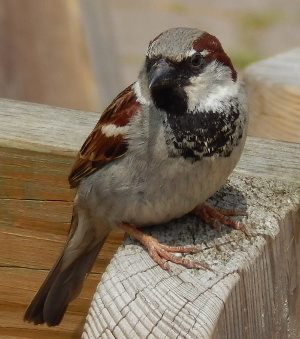
\includegraphics{images/sparrow.jpg}
\caption{\emph{Passer domesticus}}
\end{figure}

I performed an independent two-sample student's t-test on sparrow total body length to test whether or not sparrows that died in the 1898 storm were larger than sparrows that survived. I assume that both groups of sparrows (dead and living) have equal variances, so the test statistic \(t\) is calculated as follows,

\[t = \frac{\bar{X}_{1} - \bar{X}_{2}} {s_{p} \times \sqrt{\frac{1}{n_{1}} + \frac{1}{n_{2}}}}.\]

In the above, \(\bar{X}_{1}\) and \(\bar{X}_{2}\) are the mean of the samples of sparrows that died and lived, respectively. Similarly, \(n_{1}\) and \(n_{2}\) are the sample sizes of sparrows that died and lived, and \(s_{p}\) is the pooled sample mean, which is calculated as follows,

\[s_{p} = \sqrt{\frac{s^{2}_{X_{1}} + s^{2}_{X_{2}}}{2}}.\]

In the above, the \(s^{2}_{X_{1}}\) and \(s^{2}_{X_{2}}\) are the sample standard deviations for sparrows that died and lived, respectively. I conduceted the two sample t-test using the \texttt{t.test} function in R.

\clearpage

\hypertarget{references}{%
\section{References}\label{references}}

\hypertarget{refs}{}
\begin{cslreferences}
\leavevmode\hypertarget{ref-Johnston1972}{}%
1. Johnston, R. F., Niles, D. M. \& Rohwer, S. A. Hermon bumpus and natural selection in the house sparrow \emph{Passer domesticus}. \emph{Evolution} \textbf{26}, 20--31 (1972).

\leavevmode\hypertarget{ref-Darwin1859}{}%
2. Darwin, C. \emph{The origin of species}. 495 (Penguin, 1859).

\leavevmode\hypertarget{ref-Bumpus1898}{}%
3. Bumpus, H. C. Eleventh lecture. The elimination of the unfit as illustrated by the introduced sparrow, \emph{Passer domesticus}. (A fourth contribution to the study of variation.). \emph{Biological Lectures: Woods Hole Marine Biological Laboratory} 209--225 (1898).
\end{cslreferences}

\clearpage

\hypertarget{appendix-table-1}{%
\section{Appendix Table 1}\label{appendix-table-1}}

An example table is shown below, which includes all of the variables collected by \protect\hyperlink{ref-Bumpus1898}{3} for the first 10 measured sparrows. The full data set can be found online in \href{https://github.com/StirlingCodingClub/Manuscripts_in_Rmarkdown/blob/master/data/Bumpus_data.csv}{GitHub}.

\end{document}
